% article example for classicthesis.sty
\documentclass[10pt,a4paper]{article} % KOMA-Script article scrartcl
\usepackage{lipsum}
\usepackage{url}
\usepackage[nochapters]{../classicthesis} % nochapters
\usepackage{graphicx}
\usepackage{float}
\usepackage{subfig}




\begin{document}
    \pagestyle{plain}
    \title{\rmfamily\normalfont\spacedallcaps{Mission: Chuckhole | Responsibilities}}
    \author{\spacedlowsmallcaps{Michael Moosbauer}}
    \date{} % no date
    
    \maketitle
    
%    \begin{abstract}
        %Maybe we won't need an abstract
 %   \end{abstract}
       
    \tableofcontents


	

    
    \section{Introduction}
	\textbf{Mission:Chuckhole} is an Android App that provides the functionality of finding chuckholes during a bike ride. 
	The following sections briefly describe the single functionalities and the parts that have been implemented by Michael Moosbauer.


    \section{Preliminary Work}

	This section describes the work that has been done before writing the main app.
	It had to be done in order to get default values for the main app and also to get a feeling how the acceleration sensor behaves.
	
	\subsection{Acceleration Sensor Data Collection}\label{subsec:data_collection}
		
		The first step I took was to write a recording app to keep the outputs of the acceleration sensor.
		This helper app saved the values of the following form to a file:

		\begin{center}
			x;y;z;gforce
		\end{center}

		Hereby, x is the x-value, y the y-value, z the z-value from the acceleration sensor and gforce is the gforce calculated from x, y and z.
		The calculation is done the following way:

		\begin{center}
			$ gforce = \frac{\sqrt{x^2 + y^2 + z^2}}{gforce\_earth} $
		\end{center}

		The resulting file has to be placed on a computer where the program of \autoref{subsec:finding_thresholds} to be evaluated.
		The progress of evaluation is also desribed in this section.
		
	\subsection{Finding Thresholds}\label{subsec:finding_thresholds}

		In order to find suitable values for the g force that the acceleration sensor returns, I built a Java programm to evaluate the data recorded with the app described in \autoref{subsec:data_collection}.\\
		The program reads the data from a file with the format specified in the previous section.
		Over this dataset, it calculates the minimum, the maximum and the average value of all g forces.
		It can be assumed that the maximum g force value is a good approximation for finding chuckholes.\\
		Additionally, a plot for every file is generated that illustrates the distribution of g force values.
		The plot shows on the x-axis just the number of a g force and on the y-axis the values for the g force.
		The plots are shown in \autoref{fig:gforce_plots}.

		\begin{figure}[H]
	  \centering
	  \subfloat[G Force distribution for a ride on a smooth road]{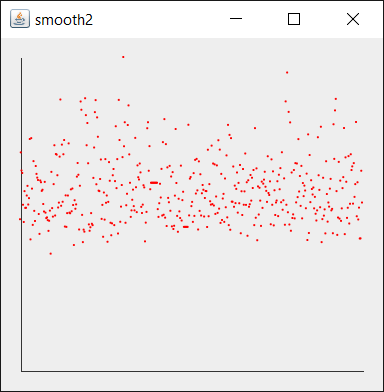
\includegraphics[width=0.4\textwidth]{img/finding_thresholds_smooth.png}\label{fig:accdist_1}}
	  \hfill
	  \subfloat[G Force distribution for a ride on cobblestones]{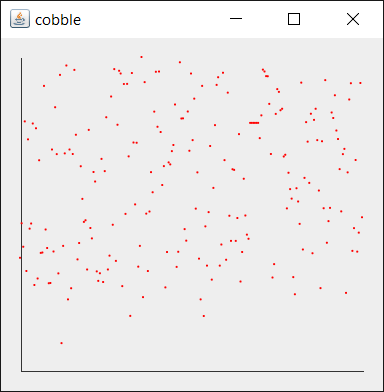
\includegraphics[width=0.4\textwidth]{img/finding_thresholds_cobble.png}\label{fig:accdist_2}}
	  \caption{G Force distribution plots}
	  \label{fig:gforce_plots}
	\end{figure}


    
    \section{System Functionalities and Responsibilities}

	This section describes the basic functionalities of the main app \textbf{Mission:Chuckhole}.



	\subsection{Onboarding}
		In case the user starts the App for the first time, he gets displayed so-called ``Onboarding'' sites.
		These sites explain the basic use of the app and are shown in \autoref{fig:onboarding}:


	\begin{figure}[H]
	  \centering
	  \subfloat[Onboarding site 1]{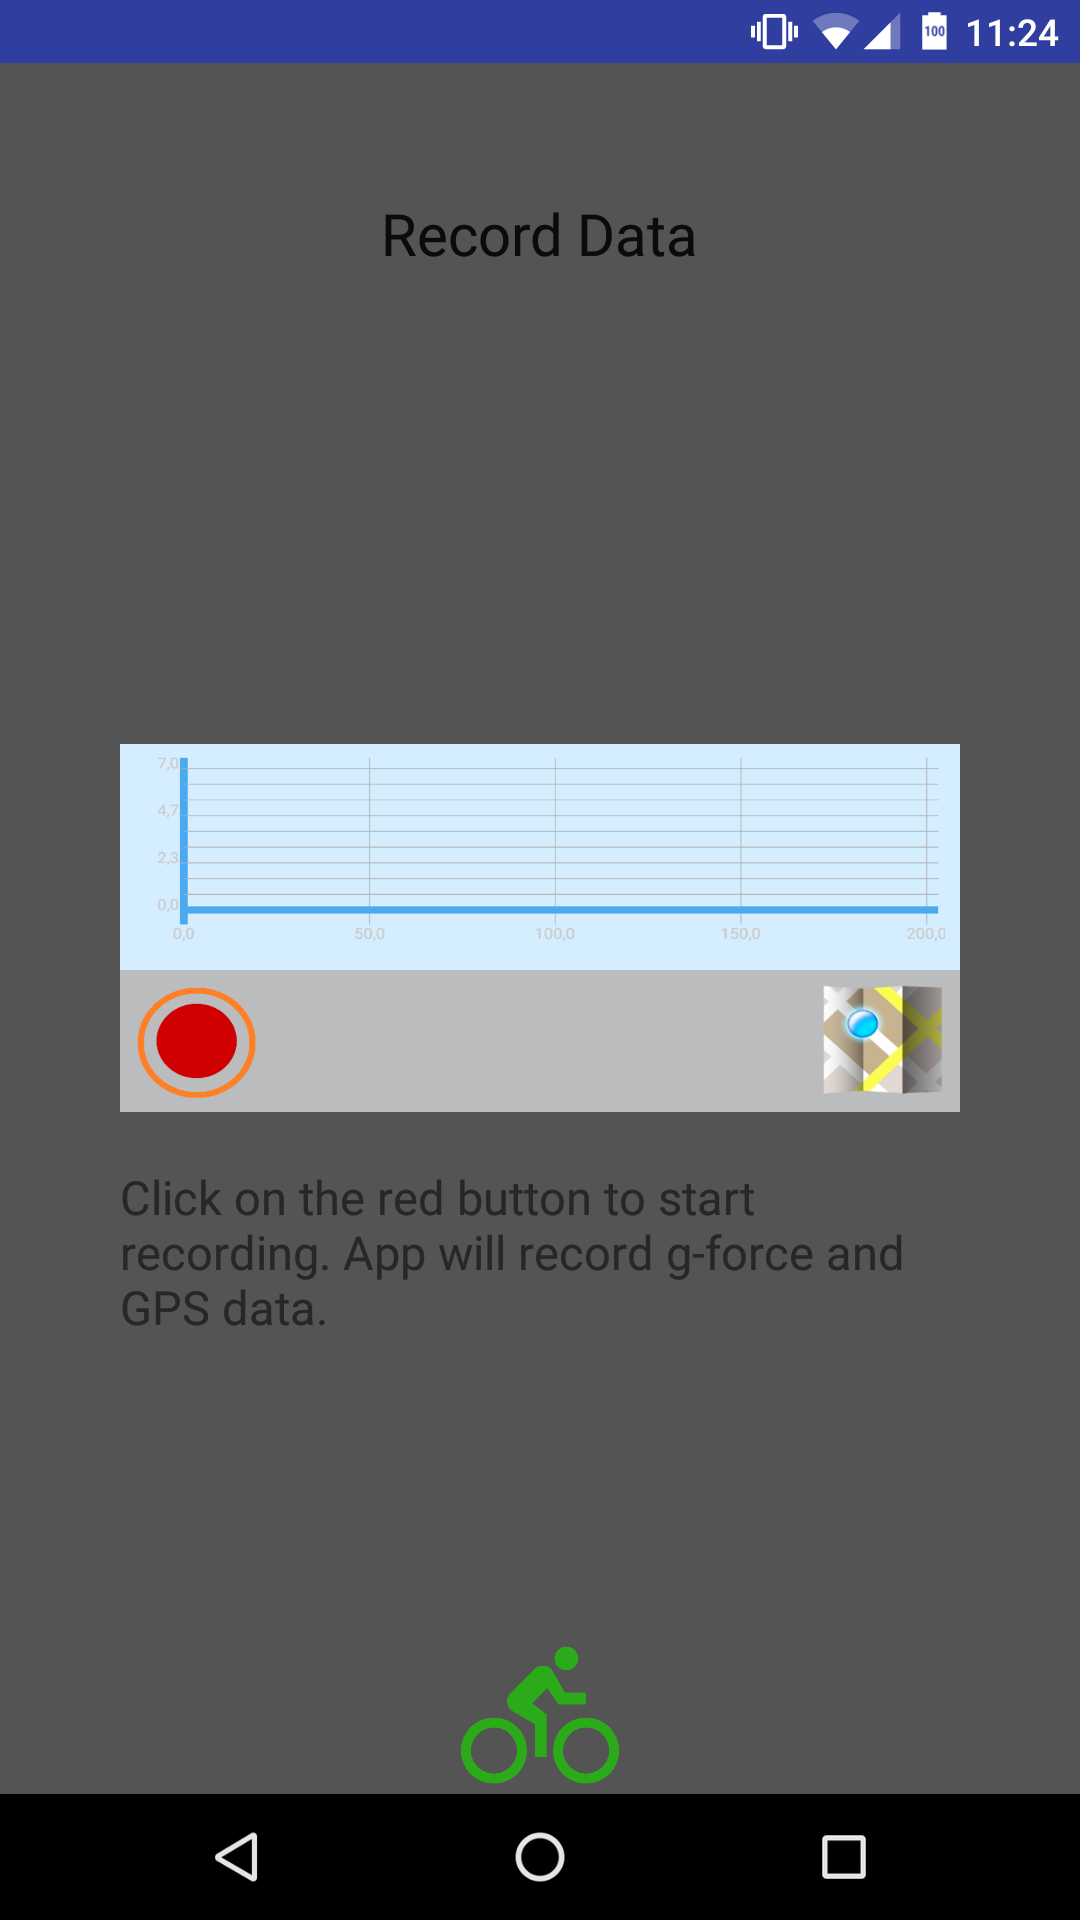
\includegraphics[width=0.25\textwidth]{img/onboarding_1.png}\label{fig:onboarding_1}}
	  \hfill
	  \subfloat[Onboarding site 2]{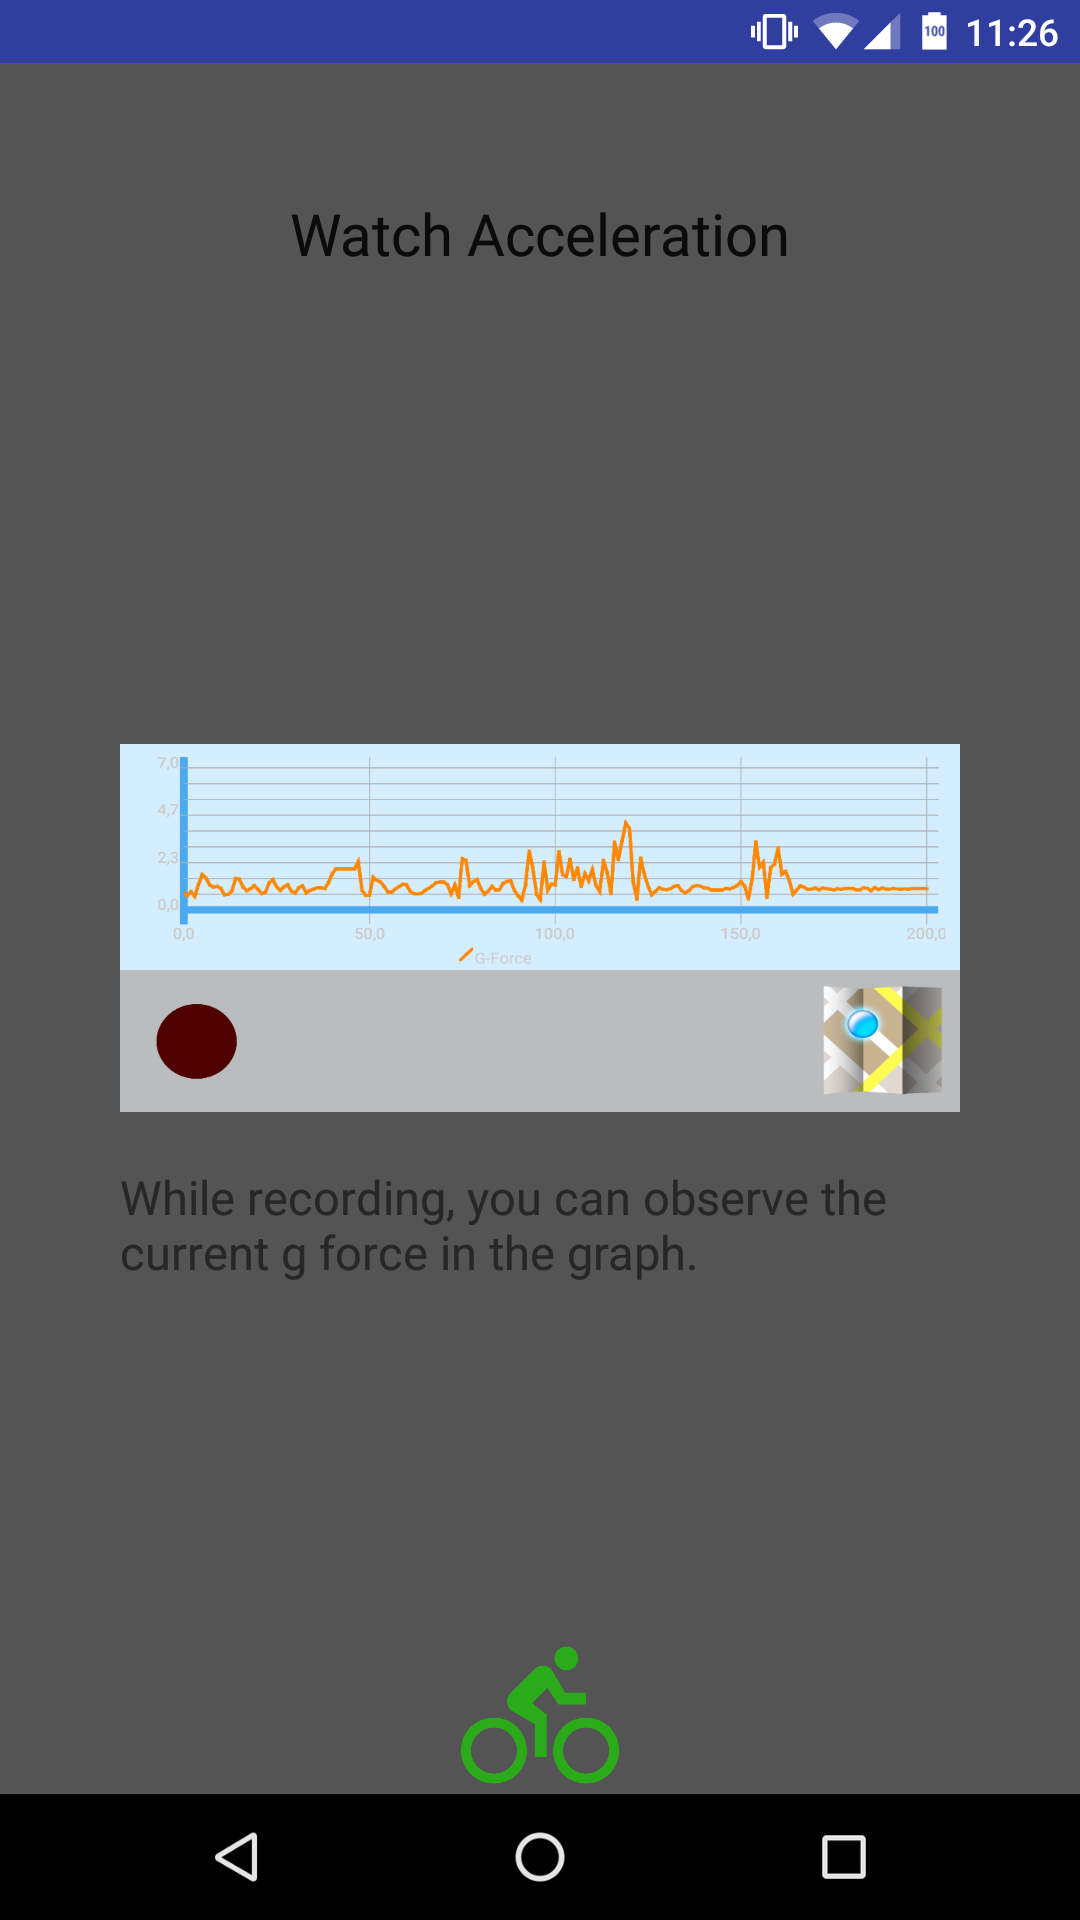
\includegraphics[width=0.25\textwidth]{img/onboarding_2.png}\label{fig:onboarding_2}}
	  \hfill
	  \subfloat[Onboarding site 3]{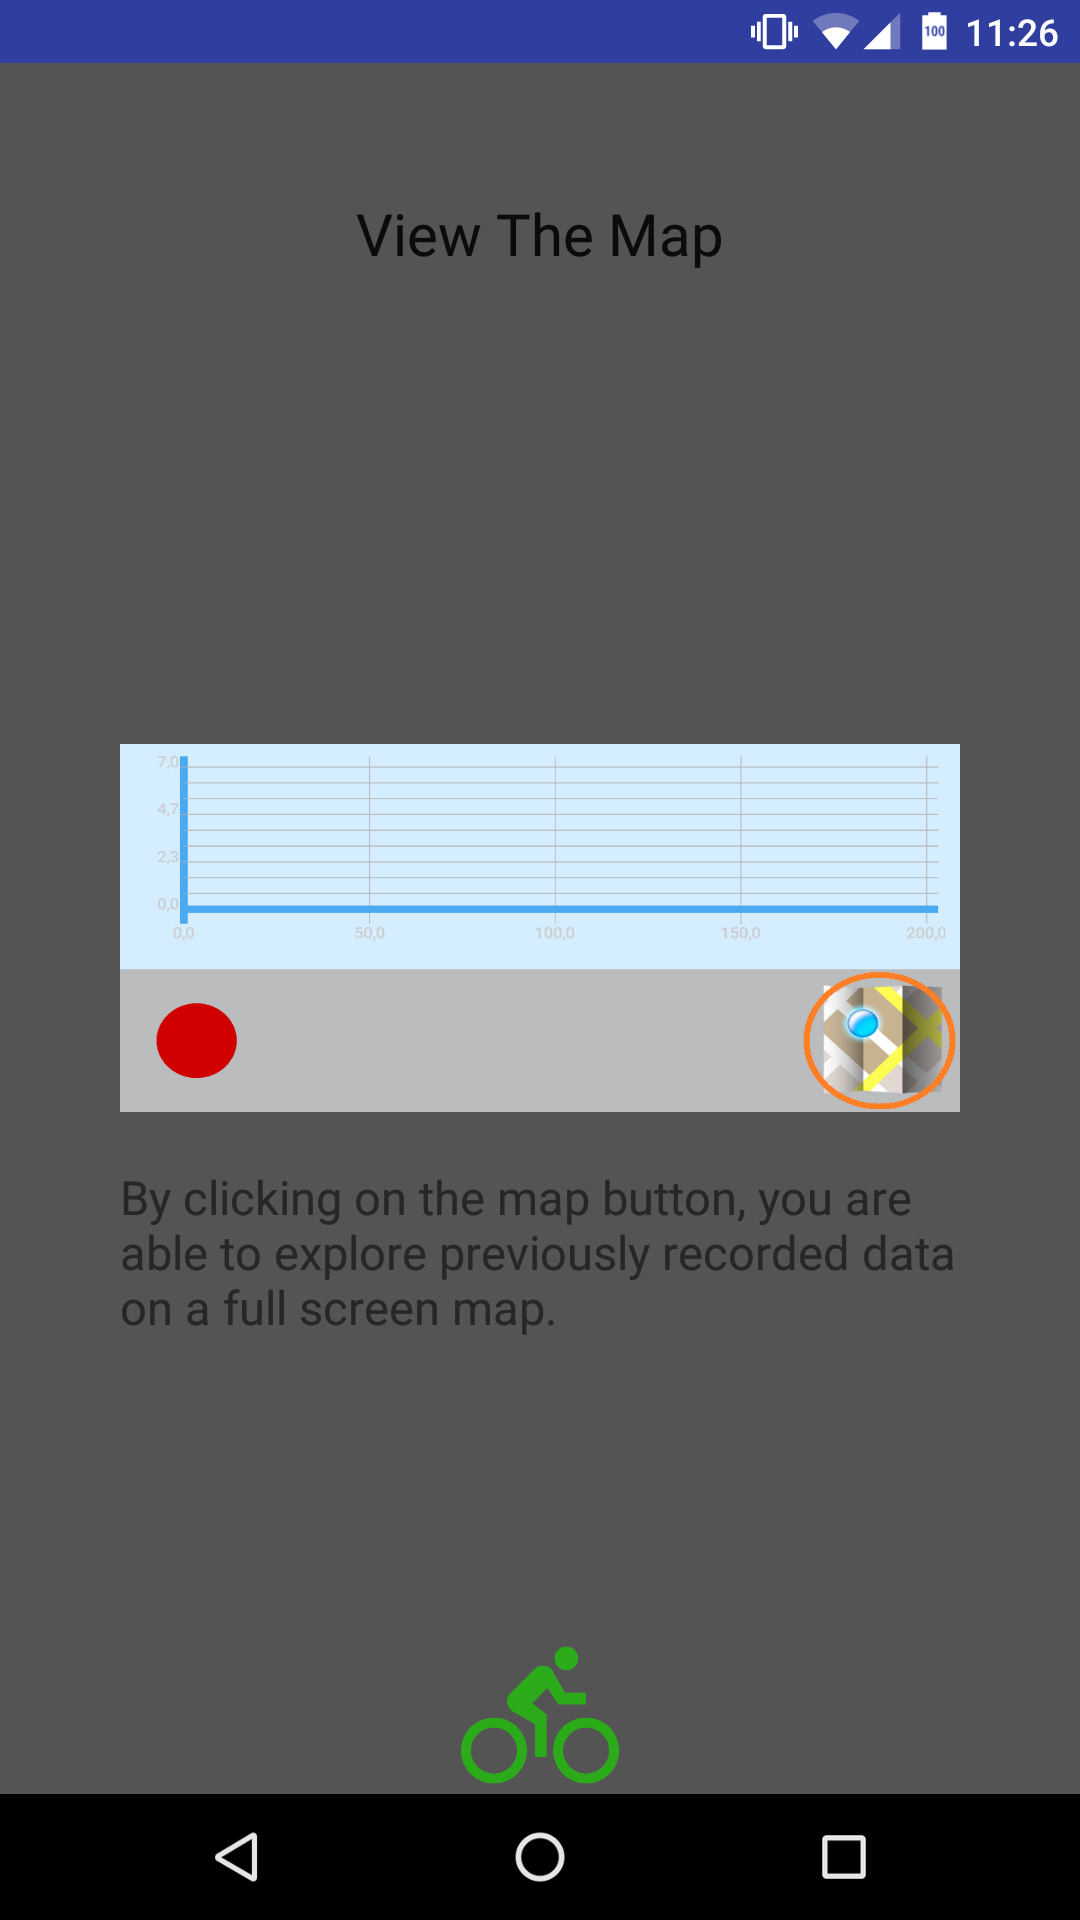
\includegraphics[width=0.25\textwidth]{img/onboarding_3.png}\label{fig:onboarding_3}}
	  \caption{Onboarding at first App start}
	  \label{fig:onboarding}
	\end{figure}





	\subsection{Start screen}
		
		\begin{figure}[H]
		\begin{center}
 		  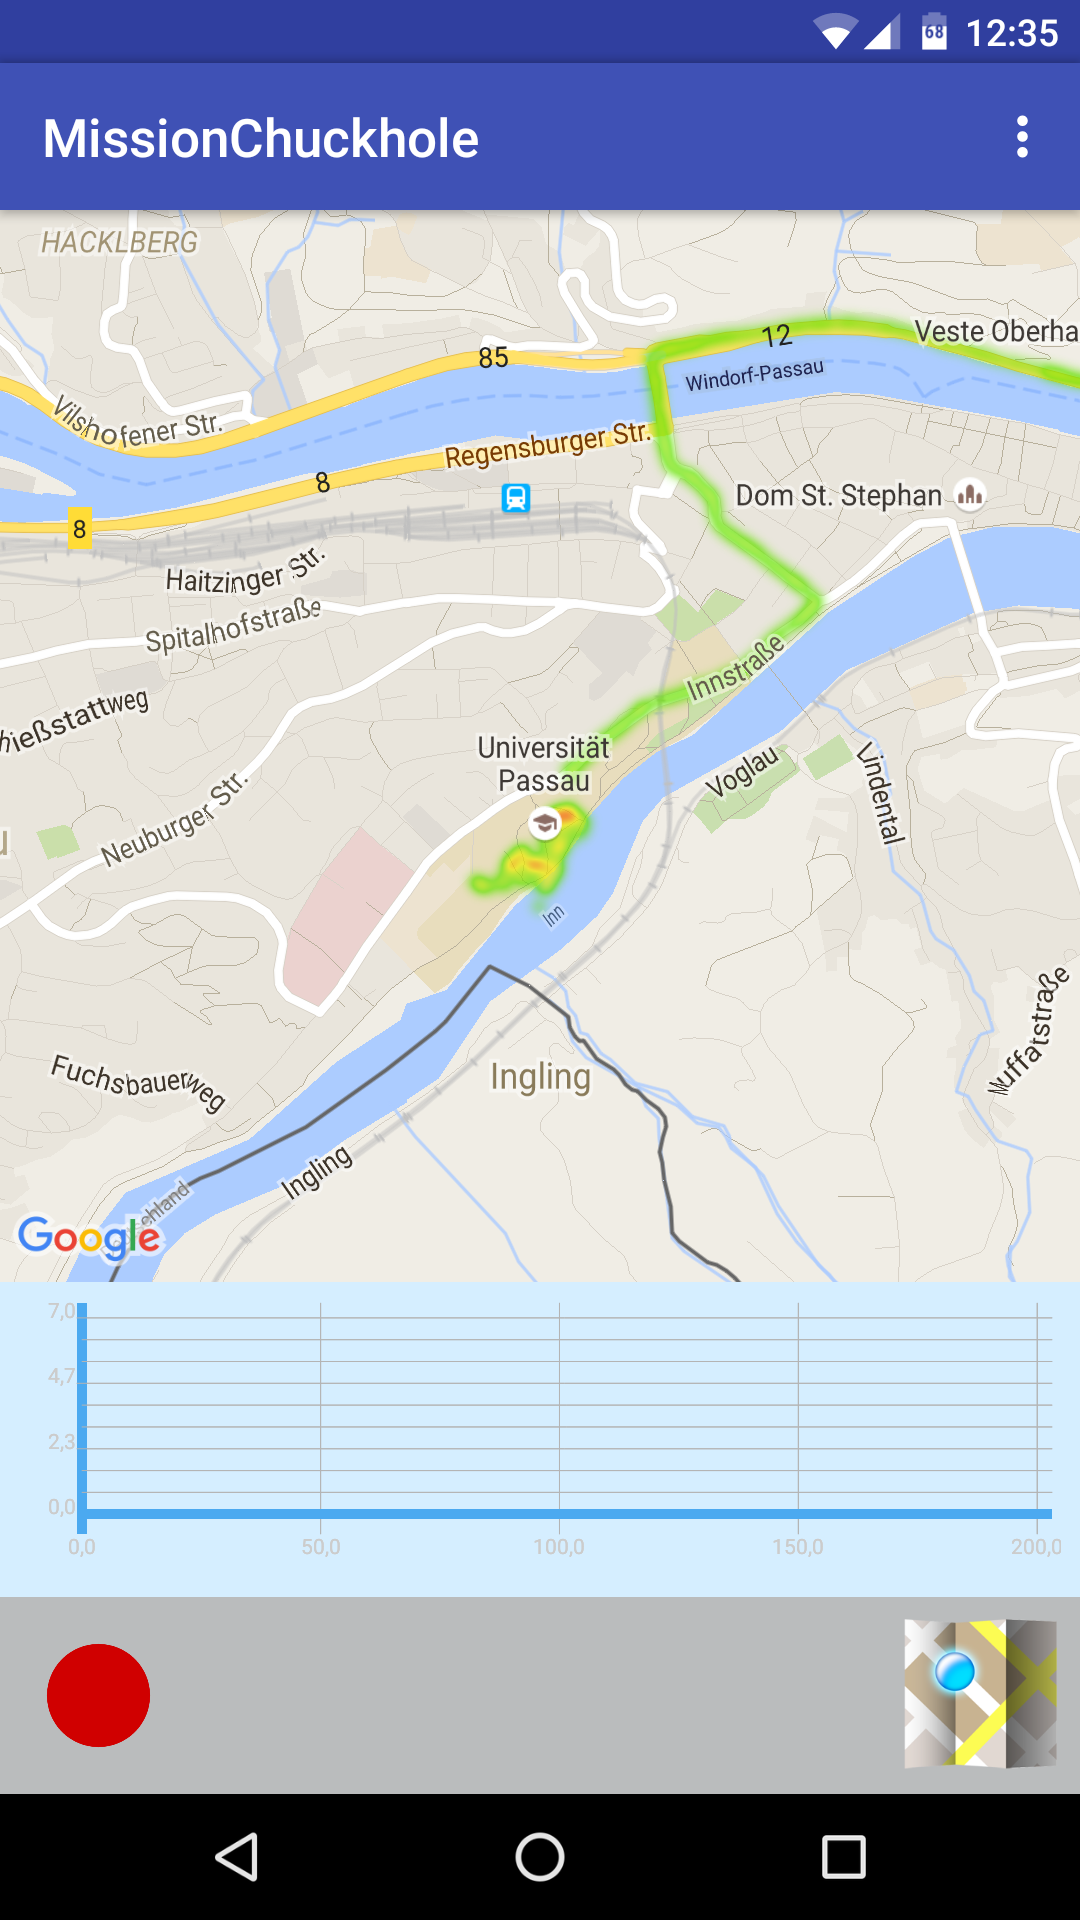
\includegraphics[scale=0.1]{img/startscreen.png}
		  \caption{Mission:Chuckhole start screen}
		  \label{fig:startscreen}
		\end{center}
		\end{figure}

	The start screen of \textbf{Mission:Chuckhole} (shown in \autoref{fig:startscreen}) consists of 			
		\begin{itemize}
			\item the Map View, moved to the current location (or University of Passau in case that no location could be provided)
			\item the Acceleration Plot View
			\item the lower bar that includes two buttons for start recording and getting to the big view of the map
		\end{itemize}

	The map view displays the current surrounding of the user as well as an overlayed heatmap that contains previously recorded data (explained in detail in \autoref{subsec:displayheatmap}).\\
	The Acceleration Plot View shows a graph of the current values for the calculated G-force while recording. 
	These values are calculated out of the x-, y- and z-values that are given from the acceleration sensor built in the smartphone and then plotted to the placeholder.\\
	The bottom bar (see \autoref{fig:bottom_bar}) is used to control the app: the right button starts the MapActivity that provides a bigger view of the map with more details.
	With the left button, recording of data is started. 
	The color of the button changes to indicate that the recording is going on.
	In the same time, the acceleration plot starts displaying the graph of G forces (see \autoref{fig:accplot}).
	While recording, clicks to the right button are disabled.\\
	
	\begin{figure}[H]
		\begin{center}
 		  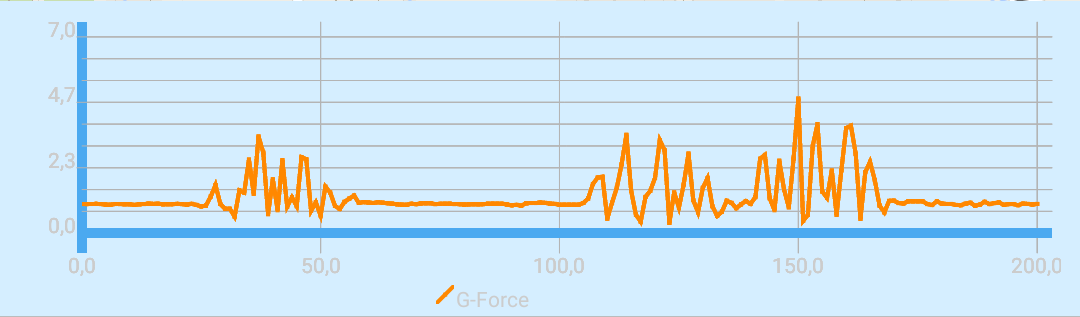
\includegraphics[scale=0.4]{img/acc_plot.png}
		  \caption{Acceleration plot running}
		  \label{fig:accplot}
		\end{center}
	\end{figure}

The following pictures illustrate the different states of recording:


	\begin{figure}[H]
	  \centering
	  \subfloat[bottom bar on startup]{
\includegraphics[width=0.4\textwidth]{img/bottom_bar_standard.png}\label{fig:bb_std}}
	  \hfill
	  \subfloat[bottom bar while recording]{
\includegraphics[width=0.4\textwidth]{img/bottom_bar_recording.png}\label{fig:bb_rec}}
	  \caption{Different states of the bottom bar}
	  \label{fig:bottom_bar}
	\end{figure}



	\subsection{Recording}

	When the record button has been pressed, a background service is started that does the whole recording.
	A SensorListener listens for updates on the acceleration sensor.
	When it gets value updates, it creates a new AccFix object which is then stored by the App DataStore (more on this can be found in \autoref{subsec:datastorage}).
	These AccFixes are only stored when valid GPS data is available, because we don't gain any information out of sensor values if we cannot map them to a valid location.
	
	
	\subsection{Displaying the heatmap}\label{subsec:displayheatmap}
	The displaying of the heatmap can be separated in two parts:

	\begin{itemize}
		\item while not recording, the data does not change, so the heatmap is displayed a single time and not updated.
		\item while recording, the data does change, so a method is invoked every ten seconds that updates the heatmap. 
	\end{itemize}

	The drawing of the heatmap just removes the previous overlay and creates a new overlay.
	The explanation why this workaround is necessary is explained in \autoref{sec:problems}.\\
	Because the GoogleMap-API heatmap uses a density approach, the dataset has to be preprocessed.
	This process (that I call ``filtering'') is explained in the next paragraph,  \autoref{subsec:filtering}.
	
	\subsection{Filtering of the dataset}\label{subsec:filtering}

	The filtering of the dataset has to be done to remove problems with the densit approach that is implemented in GoogleMap-API heatmaps.
	More details about this problem can be found in \autoref{sec:problems}.\\
	The filtering algorithm has been developed by trying and editing the found values.
	It is based on the following approach:\\
	Because the GoogleMap-API heatmaps work with a density approach, points on the heatmap are added when the map is zoomed out.
	As we are using weighted points, the single intensity add up to a new value, and higher intensity will be displayed as a more reddish point (by using the standard gradient).
	To not falsify our displaying, I created a method (DataStore.getFixes(double zoomLevel)) that returns a filtered List of AccFixes according to the handed-over zoom level.
	The filtering itself is done by the intelligent data structure ChuckDataSet, already beforce requesting data.
	Depending on the zoom level, it returns the corresponding list of AccFixes.
	The different lists contain AccFixes with different minimum distance to all other AccFixes of the list.
	The mapping of zoom level to minimum distance is shown in \autoref{tab:filtering_distances}:

	\begin{table}[H]
	  \centering
 
  
	  \begin{tabular}{c|c}
	    zoom level & minimum distance between\\
		(GooleMap value) 	& AccFixes (m)\\
	    \hline
	    	14 & 15\\
		13 & 35\\
		12 & 60\\
		11 & 250\\
		10 & 500\\
	  \end{tabular}
	   \caption{Minimum distance between AccFixes mapped to zoom levels} 
	   \label{tab:filtering_distances}
	\end{table}

	Details on how ChuckDataSet works can be found in \autoref{subsec:datastorage}. % check position

		
	\subsection{Settings}

	The settings (which can be opened by clicking the upper right button contining three dots) opens an Android SettingsActivity.
	Here, the thresholds for smooth road and cobblestones can be seen and changed.
	% TODO IMPLEMENTIEREN nach Möglichkeit!




	\subsection{Data Storage and Data Access}\label{subsec:datastorage}

	The main data type in \textbf{Mission:Chuckhole} is the \textbf{AccFix}.
	An AccFix consists of the following values:

	\begin{itemize}
		\item x: the x-value coming from the acceleration sensor
		\item y: the y-value coming from the acceleration sensor
		\item z: the z-value coming from the acceleration sensor
		\item G-force: the value for the G-force calculated from x, y and z
		\item location: the last known location of the smartphone
	\end{itemize}

	It stores the values coming from the acceleration sensor and calculates the G force out of them.
	In addition, it holds a valid GPS location to be able to map a G force value to a specific location.
	An AccFix can be converted to a String and regained from a String to simplify storing it in the database.
	This ``savestring'' is defined as follows:

	\begin{center}
		x;y;z;gforce;latitude;longitude;provider
	\end{center}
	
	Hereby, latitude and longitude define the location; the provider is a String constant for the issuer of the GPS fix.
	In this app, possible values for provider are \textbf{network} and \textbf{gps}.\\

	The data storage is basically handled by the class DataStore which is implemented as a Singleton.
	This class maintains an instance of ChuckDataSet where the AccFixes can be stored and retrieved.\\
	When AccFixes are requested (by DataStore.getFixes(double zoomLevel)), the intelligent dataset returns the according List (where the filtering has already been applied).\\
	When an AccFix is added (via DataStore.storeFix(AccFix fix)), the DataStore class calls ChuckDataSet.add(AccFix fix), which includes the whole data structure logic.
	The handed-over AccFix is handed over successively to all the add-submethods which are the following: %add new methods

	\begin{itemize}
		\item add500m(AccFix fix)
		\item add250m(AccFix fix)
		\item add60m(AccFix fix)
		\item add35m(AccFix fix)
		\item add15m(AccFix fix)
	\end{itemize}

	The number in each method indicates the minimum distance between all the AccFixes in it. 
	So each method checks if the AccFix that shall be added falls below the certain minimum distance to any other AccFix that is already in the list.
	If so, the current AccFix is not added and the method returns false; if not, it is added and the method returns true.\\

	The DataStore class also handles storing the AccFixes in a SQLite database.
	The database contains one single table \textbf{fixes} whose scheme is shown in \autoref{tab:table_scheme}.

	\begin{table}[H]
	  \centering
   
	  \begin{tabular}{c|c}
	   \_id & fix \\
	    \hline
	    	... & ...\\
	  \end{tabular}
	   \caption{Scheme for the database table ``fixes''} 
	   \label{tab:table_scheme}
	\end{table}

	\textbf{\_id} is an auto-incrementing field that is only needed for proper storing.
	The values in the \textbf{fixes}-column hold the AccFixes as savestrings as explained at the beginning of this section.
	
	\section{Problems/Lessons Learned}\label{sec:problems}

	Some problems occured during implementation that could be solved quite well.\\
	The first one was the heatmap density problem.
	I recognized this problem while zooming the map on the start screen: the recorded data (which was first tested in a car on a smooth road) was shown well in a nice green in high zoom levels, but on zooming out, the heatmap was shwon more and more reddish.
	This effect was issued by the GoogleMap-API heatmap's behaviour on zooming: if the user zooms out, points with a small distance are summed up to a single point.
	While we use weighted heatmaps (this way, we can take control of the coloring of different G-force values), the intensities of all the points are added up and result in a much bigger value than the single values have been.
	To get rid of this behaviour, I added the filtering algorithm described in \autoref{subsec:filtering}.\\

	Another problem occurred when updating the heatmap while recording (mentioned in \autoref{subsec:displayheatmap}).
	The standard way to update a heatmap overlay would be just to hand over the new data to the TileProvider used to create the overlay and then tell the overlay to clear its tile cache so that the updated data is loaded.
	Unfortunately, this caused flickering of the heatmap and ended up in displaying the heatmap in only very few cases.





    
    % bib stuff
    \nocite{*}
    \addtocontents{toc}{\protect\vspace{\beforebibskip}}
    \addcontentsline{toc}{section}{\refname}    
    \bibliographystyle{plain}
    \bibliography{../Bibliography}
\end{document}